\documentclass[11pt,letterpaper]{article}
\usepackage{geometry}
\geometry{margin=1in}

\usepackage{graphicx}
\usepackage{caption}   % for better caption control
\usepackage{float}     % to control image placement
\usepackage{parskip}   % to add spacing between paragraphs
\usepackage[hidelinks]{hyperref}
\usepackage{amsmath}
\usepackage{amsmath}
\usepackage{amsfonts} 
\usepackage{minted}
\usepackage{mathtools}
\usepackage{cancel}
\usepackage{subcaption}
\usepackage[thinc]{esdiff}
\usepackage{listings}
\usepackage[framed , numbered]{matlab-prettifier}
\usepackage{bm}
\usepackage{graphicx}
\usepackage{siunitx}
\usepackage{tikz}
\usepackage{booktabs}
\usepackage{hyperref}
\usepackage{tabularx}
\usepackage{url}

\setlength{\parindent}{0pt}
\setlength{\parskip}{0.5em}

% Lists and spacing
\usepackage{enumitem}
\setlist{nosep}

% Reduce section spacing
\usepackage{titlesec}
\titlespacing*{\section}{0pt}{0\baselineskip}{0.5\baselineskip}
\titlespacing*{\subsection}{0pt}{0\baselineskip}{0.3\baselineskip}
\titlespacing*{\subsubsection}{0pt}{0\baselineskip}{0.3\baselineskip}

\title{Lab 3.1 - FMRI, Stat 214, Spring 2025\vspace{-1em}}
\author{Anonymous}

% submission must not contain any of your names
% but feel free to make a version for yourself with your names on it
% \author{Your names}

\begin{document}
\maketitle

\vspace{1em} % space before
\section{Introduction}
\vspace{0.5em} % space after
Understanding how the brain processes language is a key challenge in both neuroscience and artificial intelligence. In natural settings, humans interpret language as a continuous stream of words that unfold over time. The brain must rapidly extract meaning from this input using both current and past context. Functional magnetic resonance imaging (fMRI) provides a non-invasive way to study this process by measuring brain activity in response to natural speech. In this lab, our aim is to model these responses using computational text representations.

The central goal of this lab is to evaluate the ability of language embeddings to predict brain activity recorded by fMRI. We do this by constructing voxel-wise encoding models, which take as input a sequence of word-level embeddings and output predicted brain responses. We compare 3 types of embedding, including Bag-of-Words,  Word2Vec and GloVe, to assess their ability to explain variance in neural signals. These embeddings differ in the extent to which they capture the semantic structure and temporal context.

We focus on data collected from two human subjects who listened to a set of narrated stories while undergoing fMRI scanning. Each story is accompanied by a time-aligned transcript. The transcripts are processed into numerical representations using various embedding techniques. These embeddings are then aligned with the fMRI time series and used as input features for regression models. The models are trained to predict the BOLD signal measured in each voxel of the brain.

Our analysis builds on previous work that showed context-aware embeddings improve encoding performance (Jain \& Huth, 2018). These results suggest that the brain integrates meaning over time, rather than processing each word independently. By comparing the predictive accuracy of models trained on different embeddings, we test this hypothesis and identify regions of the brain that are sensitive to the semantic and contextual features of language.

From a statistical perspective, this lab provides a framework for studying high-dimensional regression problems in neuroscience. It involves regularization, time series alignment, and model evaluation in tens of thousands of responses. More broadly, the work contributes to understanding how language models used in natural language processing relate to brain function during real-world language comprehension.

\vspace{1em} % space before
\section{Generating Embeddings}
\vspace{0.5em} % space after
To model the brain's response to language, we first converted raw text from each podcast into numerical embeddings. These embeddings serve as input features (\texttt{X}) for predicting the fMRI BOLD response (\texttt{Y}). The embedding techniques used include Bag-of-Words (BoW), Word2Vec, and GloVe. For each of these embedding techniques, the available story data was split into training and test sets.

\vspace{1em} % space before
\subsection{Bag-of-words Embedding}
\vspace{0.5em} % space after
For the BoW approach, \texttt{CountVectorizer} from \texttt{sklearn} was used to build a vocabulary with stop words removed. Essentially, this helps us construct a vocabulary of unique words and transforms each word into a high-dimensional sparse vector that counts the frequency of each vocabulary word. Therefore, each story is represented as a sequence of word-count vectors.

However, the embeddings initially generated are at the word level, meaning there is one embedding vector per word. This means that the resolution is too high when compared to the fMRI response, which was collected at a much lower frequency -- approximately once per second. To align the dimensions between our embeddings and the fMRI BOLD signal, we applied downsampling from the provided preprocessing script. This aggregates the word-level embeddings to more closely align with the time resolution in the BOLD signal.

To finalize alignment and also reduce boundary effects, we trimmed the first 5 seconds and last 10 seconds from each downsampled embedding matrix. After the downsampling, we assumed a 1-second interval per row. After this trimming, the BoW embeddings resolution now exactly matched that of the BOLD signal.

The last step of generating the embeddings involved creating lagged versions using the \texttt{make\_delayed} function from the preprocessing script. Brain responses are not instantaneous since there is a delay between hearing words and the corresponding neural activity. To account for this lag, delays from 1 to 4 seconds were applied to the trimmed and downsampled embeddings. After applying this, it means that the model now has access to the embeddings from the previous 1 to 4 seconds, allowing it to use past context to better predict the current brain response.

\vspace{1em} % space before
\subsection{Word2Vec Embedding}
\vspace{0.5em} % space after
For the Word2Vec approach, we used the pre-trained \texttt{word2vec-google-news-300} model available through Gensim. This model provides dense 300-dimensional vector representations of words, trained on the Google News corpus. Each word in each story transcript was mapped to its corresponding Word2Vec vector. If a word was not found in the model’s vocabulary, we assigned a zero vector of length 300.

After converting each word into its vector representation, we obtained a sequence of word-level embeddings for each story. Since these embeddings are generated at the word level, they do not naturally align with the slower temporal resolution of the fMRI BOLD signal. To address this mismatch, we used the \texttt{downsample\_word\_vectors} function from the provided preprocessing script. This step aggregated the high-frequency word embeddings into vectors aligned with the timing of the fMRI scans, typically at one sample per second.

As with the other embedding methods, we trimmed the first 5 seconds and the last 10 seconds from the downsampled embeddings. This trimming helps remove potential boundary effects and ensures that the embedding and BOLD matrices have compatible dimensions for modeling. After this step, each story’s embedding matrix had the same number of rows as its corresponding trimmed fMRI response matrix.

To further account for the temporal dynamics of neural processing, we applied the \texttt{make\_delayed} function with delays ranging from 1 to 4 seconds. This created lagged versions of the embeddings, allowing the model to incorporate recent contextual information. The final embedding matrix for each story had $300 \times 4 = 1200$ features per timepoint, with each feature representing the embedding from a different delay. These lagged embeddings were then used as the input features for the ridge regression models.


\vspace{1em} % space before
\subsection{GloVe Embedding}
\vspace{0.5em} % space after

For the GloVe approach, we used the pre-trained \texttt{glove-wiki-gigaword-300} embeddings, which provide 300-dimensional vector representations for a wide range of English words based on co-occurence statistics from a large corpus. Each word in each story was mapped to its corresponding GloVe vector, and words not found in the pre-trained vocabulary were assigned a zero vector. This transformed each story into a sequence of dense word embeddings, where each word is represented by its semantic properties in vector space, rather than by its frequency, like in BoW.

As with BoW and Word2Vec, the resulting embeddings were at the word level, which is at a much higher resolution that the fMRI BOLD signal. To align the embeddigs with the fMRI data, we again used downsampling.

We then trimmed the first 5 seconds and last 10 seconds from each downsampled GloVe matrix to ensure alignment with the BOLD signal and to reduce edge-related noise. 

Finally, we applied the \texttt{make\_delayed} function with delays ranging from 1 to 4 seconds. This created lagged versions of the embeddings, allowing the model to incorporate context from the previous 1 to 4 seconds when predicting the brain's current response. 

\vspace{1em} % space before
\subsection{Benefits of Pre-trained Embeddings}
\vspace{0.5em} % space after
Pre-trained embeddings provide several advantages when modeling brain responses to natural language. Unlike frequency-based methods, these embeddings capture richer linguistic features and allow more effective learning from limited neural data.

One of the main benefits is the semantic structure learned from large-scale corpora. Pre-trained embeddings such as Word2Vec and GloVe are trained on billions of words from diverse sources. They represent words in a continuous vector space where proximity reflects semantic similarity (e.g., \textit{king} and \textit{queen} have similar vectors). This semantic information may correspond to cognitive processes in the brain, potentially making these embeddings more ``brain-like'' compared to frequency-based alternatives.

Another key advantage is data efficiency. fMRI datasets are high-dimensional but typically contain a limited number of training samples due to cost and logistical constraints. Pre-trained embeddings reduce the need to learn representations from scratch, providing a strong prior over the input space. This helps mitigate overfitting in downstream regression models.

Additionally, pre-trained embeddings produce dense and compact representations, which are computationally more efficient than sparse alternatives. This is especially useful when applying linear models, such as ridge regression, to tens of thousands of voxels, each with potentially thousands of timepoints.

Finally, using standardized pre-trained embeddings across models ensures comparability. Since each embedding method outputs fixed-dimensional vectors (e.g., 300-dimensional), we can directly compare their performance in predicting neural responses. This facilitates benchmarking and helps to evaluate which embedding aligns best with the structure of brain activity.

\begin{table}[htbp]
\centering
\small
\caption{Comparison of Embedding Methods}
\begin{tabular}{l|c|c|c}
\toprule
\textbf{Property} & \textbf{BoW} & \textbf{Word2Vec} & \textbf{GloVe} \\
\midrule
Representation & Sparse & Dense & Dense \\
Pre-trained & No & Yes & Yes \\
Semantic Info & No & Yes & Yes \\
Context Capture & No & Partial & Partial \\
Dimensionality & High & 300 & 300 \\
Comp. Cost & Low & Moderate & Moderate \\
Efficiency & Low & High & High \\
Brain Alignment & Weak & Moderate--Strong & Moderate \\
\bottomrule
\end{tabular}
\end{table}


\newpage
\vspace{1em} % space before
\section{Modeling}
\vspace{0.5em} % space after

Three ridge regression models -- one for each embedding type (Bag-of-Words, Word2Vec, and GloVe) -- were trained using the aligned and lagged feature matrices derived from the podcast transcripts. Each model was trained on a combined dataset of multiple stories, with the embeddings used to predict the voxel-wise BOLD responses recorded via fMRI. A fixed regularization parameter (alpha = 100) was initially chosen across all models to allow for a fair comparison of embedding effectiveness. Each model was evaluated on a held-out test set composed of different stories not used during training.

To account for temporal misalignment between the text and brain response, embeddings were downsampled and trimmed at the start and end. Additionally, lagged versions of the features were created to capture delayed neural responses to language. The performance of each model was measured using correlation coefficients (CC) between predicted and actual fMRI signals at each voxel. We report the mean, median, and top percentile CCs as primary evaluation metrics.

While alpha was not tuned individually for each embedding, a cross-validation analysis on the best-performing embedding is conducted later to explore the impact of regularization. A stability analysis is also included to assess generalization across subjects and stories.

\vspace{1em} % space before
\subsection{Bag-of-Words (BoW) Ridge Regression}
\vspace{0.5em} % space after

The first ridge regression model was trained using Bag-of-Words (BoW) embeddings derived from the raw podcast transcripts. Each word was represented as a one-hot vector, resulting in a high-dimensional but sparse feature matrix. After aligning the word embeddings with the fMRI timepoints via downsampling and trimming, lagged features were generated with delays ranging from 1 to 4 seconds to capture delayed neural responses. Due to missing fMRI recordings, a few stories were excluded from both the training and testing sets. The final training data consisted of 28,644 timepoints and 43,916 features across all usable stories.

The model's performance was evaluated on held-out test stories using voxel-wise Pearson correlation coefficients (CC) between predicted and actual BOLD signals. As shown in Figure \ref{fig:prob_hist_bow}, the resulting CC distribution was centered near zero, with a mean CC of 0.0017 and a median of 0.0016. Only a small subset of voxels showed modest predictive performance, with the top 1\% and top 5\% reaching 0.0329 and 0.0234, respectively. These results suggest that while BoW captures some minimal information about brain responses to language, its simplistic representation may lack the semantic richness required for accurate neural encoding.

\begin{table}[H]
\centering
\begin{tabular}{lcccc}
\toprule
\textbf{} & \textbf{Value} \\
\midrule
Mean CC    & 0.0017 \\
Median CC  & 0.0016 \\
Top 1\% CC & 0.0329 \\
Top 5\% CC & 0.0234 \\
\bottomrule
\end{tabular}
\caption{BoW Ridge Regression Model Performance (Subject 2)}
\label{tab:bow_cc_results}
\end{table}

\begin{figure}[ht]
    \centering
    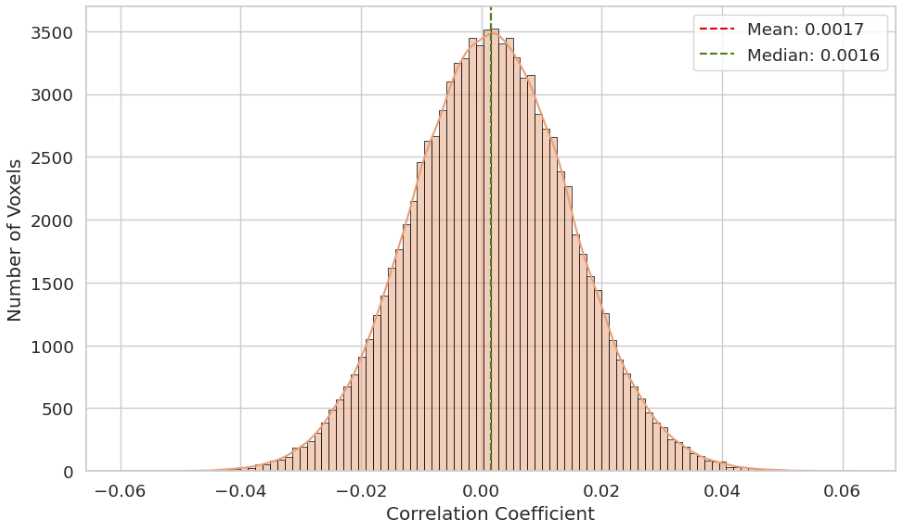
\includegraphics[width=0.9\textwidth]{figs/cc-dist-bow.png}
    \caption{Bag-Of-Words Correlation Coefficient Distribution}
    \label{fig:prob_hist_bow}
\end{figure}

\vspace{1em} % space before
\subsection{Word2Vec Ridge Regression}
\vspace{0.5em} % space after

To explore the benefits of semantically enriched representations, a ridge regression model was trained using pre-trained Word2Vec embeddings from the Google News corpus. Each word in the transcript was mapped to a 300-dimensional vector, and embeddings were aligned with the fMRI recordings through downsampling, trimming, and temporal lagging. After removing timepoints associated with NaN values in the fMRI signal, the final training set consisted of 27,867 timepoints and 1,200 input features. The model was saved for reproducibility and later evaluation.

The model's performance was again evaluated using voxel-wise Pearson correlation coefficients on held-out test stories. As shown in Figure \ref{fig:prob_hist_w2v}, the distribution of CC values remained tightly centered around zero, but with slightly higher values than the Bag-of-Words model. The mean CC was 0.0039 and the median was 0.0036, indicating marginally improved predictive performance. Notably, the top 1\% and top 5\% of voxels achieved CCs of 0.0410 and 0.0284, respectively. While the overall predictive power is still weak, the improvement over BoW suggests that Word2Vec captures a modest degree of neural-relevant semantic information. However, most voxels remained poorly predicted, which may reflect either noise in the data, insufficient modeling capacity, or the need for more task-specific embeddings.

\begin{table}[H]
\centering
\begin{tabular}{lcccc}
\toprule
\textbf{} & \textbf{Value} \\
\midrule
Mean CC    & 0.0039 \\
Median CC  & 0.0036 \\
Top 1\% CC & 0.0410 \\
Top 5\% CC & 0.0284 \\
\bottomrule
\end{tabular}
\caption{Word2Vec Ridge Regression Model Performance (Subject 2)}
\label{tab:w2v_cc_results}
\end{table}

\begin{figure}[h]
    \centering
    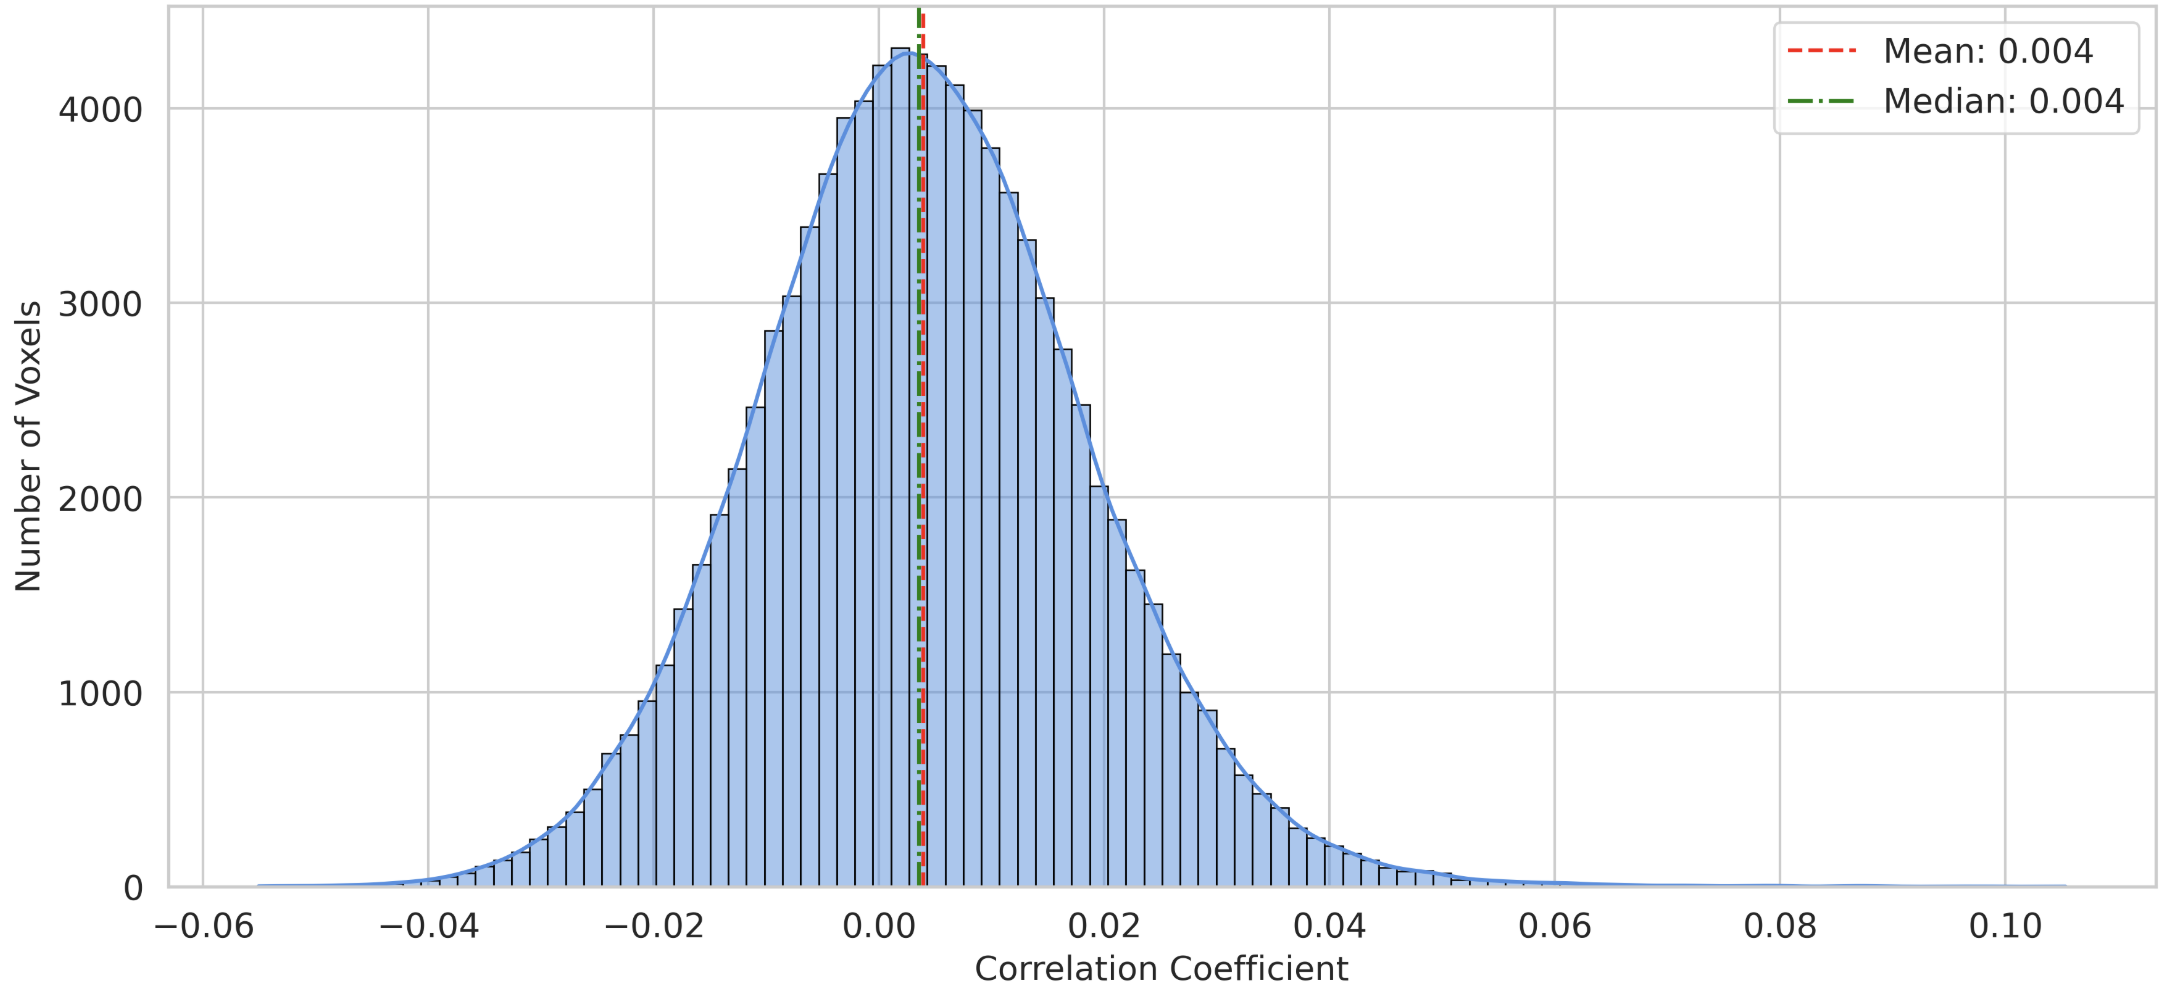
\includegraphics[width=0.9\textwidth]{figs/cc-dist-word2vec.png}
    \caption{Word2Vec Correlation Coefficient Distribution}
    \label{fig:prob_hist_w2v}
\end{figure}

\vspace{1em} % space before
\subsection{GloVe Ridge Regression}
\vspace{0.5em} % space after

The third model utilized GloVe embeddings trained on the Common Crawl corpus to represent the transcript text. Each word was mapped to a 300-dimensional vector, and the aligned embeddings were downsampled, trimmed, and temporally lagged to match the BOLD fMRI signal across time. As with the other models, several stories were excluded due to missing voxel recordings. The final training dataset consisted of 28,644 timepoints and 1,200 lagged input features.

Model performance was evaluated on held-out stories using voxel-wise Pearson correlation coefficients. As shown in Figure \ref{fig:prob_hist_glove}, the distribution of CCs remained centered near zero but demonstrated the strongest predictive performance among all three embedding methods. The model achieved a mean CC of 0.0049 and a median of 0.0044. Top-performing voxels reached a CC of 0.0441 in the top 1\% and 0.0302 in the top 5\%.

Compared to BoW and Word2Vec, the GloVe-based model consistently produced higher CC values across the voxel distribution. This suggests that GloVe’s co-occurrence-based training objective and use of global corpus statistics may lead to richer semantic representations that align more effectively with brain activity patterns. GloVe's ability to capture both syntactic and semantic regularities—while being less sensitive to local word order—may be particularly advantageous for modeling long-form, spoken language like podcasts. Although the overall CCs remain low, GloVe shows the most promise among the tested embeddings for linking linguistic content to neural responses in this dataset.

\begin{table}[H]
\centering
\begin{tabular}{lcccc}
\toprule
\textbf{} & \textbf{Value} \\
\midrule
Mean CC    & 0.0049 \\
Median CC  & 0.0044 \\
Top 1\% CC & 0.0441 \\
Top 5\% CC & 0.0302 \\
\bottomrule
\end{tabular}
\caption{GloVe Ridge Regression Model Performance (Subject 2)}
\label{tab:glove_cc_results}
\end{table}

\begin{figure}[h]
    \centering
    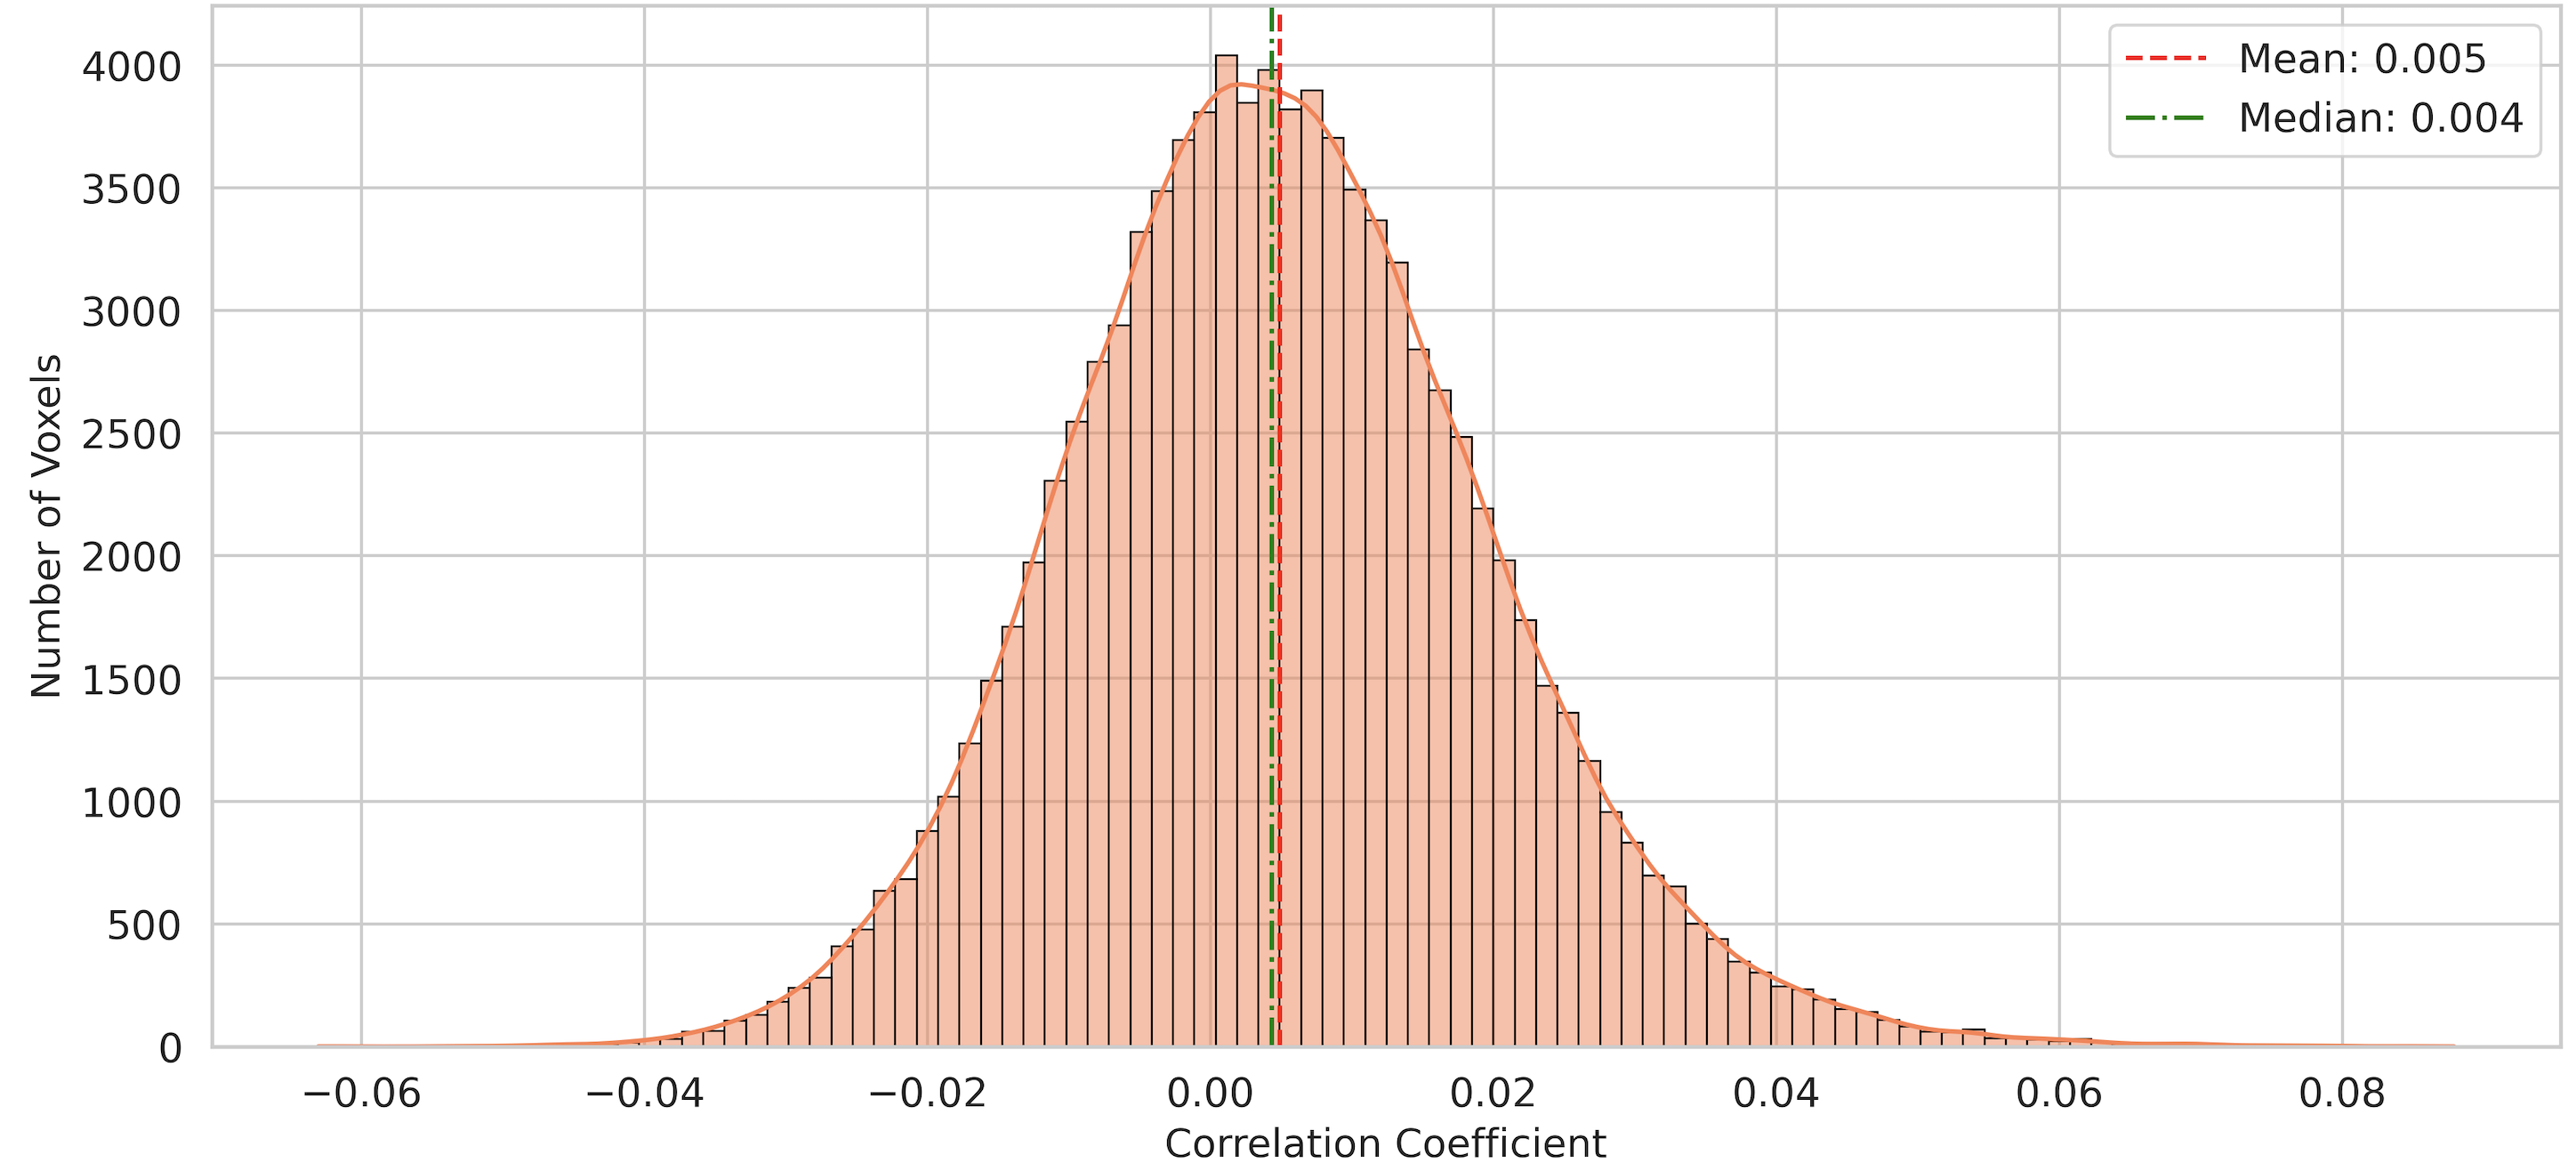
\includegraphics[width=0.9\textwidth]{figs/cc-dist-GloVe.png}
    \caption{GloVe Correlation Coefficient Distribution}
    \label{fig:prob_hist_glove}
\end{figure}

\vspace{1em} % space before
\subsection{The Best Embedding Model}
\vspace{0.5em} % space after

In this section, we compare the performance of three different text embeddings—Bag-of-Words (BoW), Word2Vec, and GloVe—in predicting brain activity from podcast text. The models were evaluated based on four key metrics: Mean CC, Median CC, Top 1\% CC, and Top 5\% CC.

The results of our comparison show that GloVe outperforms both BoW and Word2Vec in all metrics, with the highest Mean CC of 0.0049 before adjusting the regularization parameter, and 0.0083 after tuning the alpha parameter. This indicates that GloVe provides more accurate predictions of voxel-wise brain activity correlations. Specifically, the Mean CC for BoW was 0.0021, and for Word2Vec, it was 0.0039, both lower than GloVe. Additionally, GloVe achieved the highest Median CC of 0.0044 before optimization, which improved to 0.0068 after adjusting alpha.

One of the most notable improvements after adjusting alpha was observed in the Top 1\% CC, where GloVe increased from 0.0441 to 0.0622. This shift indicates that the model now better captures the strongest correlations between podcast text and brain activity. Similarly, for the Top 5\% CC, GloVe improved from 0.0302 to 0.0392, suggesting a more robust model that is better able to predict the top-performing voxels in the brain.

The distributions of the voxel-wise correlation coefficients further highlight these improvements. As shown in the accompanying histograms, the Before tuning distribution had a more concentrated peak around a Mean CC of 0.0049 and Median CC of 0.0044 (Figure 1). However, after tuning the alpha parameter, the After tuning distribution shifted, showing a wider range with a higher peak around the new Mean CC of 0.0083 and Median CC of 0.0068 (Figure 2). This suggests that, with the optimized alpha, the model's performance across the voxels became more consistent, with a noticeable increase in the number of voxels exhibiting higher correlation coefficients.

\begin{table}[ht]
\centering
\begin{tabular}{|c|c|c|}
\hline
\textbf{Metric} & \textbf{Before Tuning} & \textbf{After Tuning} \\
\hline
Mean CC & 0.0049 & 0.0083 \\
\hline
Median CC & 0.0044 & 0.0068 \\
\hline
Top 1\% CC & 0.0441 & 0.0622 \\
\hline
Top 5\% CC & 0.0302 & 0.0392 \\
\hline
\end{tabular}
\caption{Comparison of CC Results}
\end{table}

These results suggest that adjusting the alpha parameter not only improves the overall performance of GloVe but also increases its ability to capture stronger and more meaningful relationships between the podcast text and brain activity. GloVe has therefore been selected as the best embedding model for predicting brain voxel responses from podcast text. Future work may involve further fine-tuning the GloVe model or exploring advanced embeddings to enhance predictive accuracy.


\vspace{1em} % space before
\subsection{Stability Check}
\vspace{0.5em} % space after

In this section, we evaluate the stability of the ridge regression model's predictions across different test stories by analyzing voxel-wise correlation coefficients (CCs). The violin plot in Figure \ref{fig:violin_glove} represents the distribution of CCs for each of the 19 test stories. The x-axis corresponds to the test stories, labeled from "Story 1" to "Story 19," and the y-axis represents the correlation coefficient, which measures the strength of the relationship between the predicted and actual voxel responses. The width of the violins indicates the distribution of CCs, with thicker regions showing the more common values. The black bars inside the violins represent the interquartile range (IQR), and outliers are shown as red points, which indicate cases where the model's predictions deviate significantly from the actual responses.

The plot reveals that the model’s performance is relatively consistent across most test stories, with the majority of stories having narrow violin shapes. This indicates that the model’s predictions are fairly stable, with the CCs for most test stories clustering around similar values. The median CC for most stories appears to be close to 0, suggesting weak correlations between the model's predictions and the actual FMRI data. The relatively narrow distributions for these stories further imply that the model performs similarly across these test stories. However, there are a few stories where the violin plots are wider, indicating more variability in the model's performance. These wider distributions suggest that for some stories, the model's performance is less stable, with more fluctuation in the predicted voxel responses.

In conclusion, the model is generally stable across most test stories, but there are a few test stories where the model shows instability in its predictions, as evidenced by the wider distributions and outliers. The presence of these outliers, which represent stories where the CCs are lower than expected, indicates that the model struggles with some specific test stories. This variability highlights areas where the model could be improved, either by refining the feature extraction process or tuning the model parameters to better generalize across all types of test stories.

\begin{figure}[h]
    \centering
    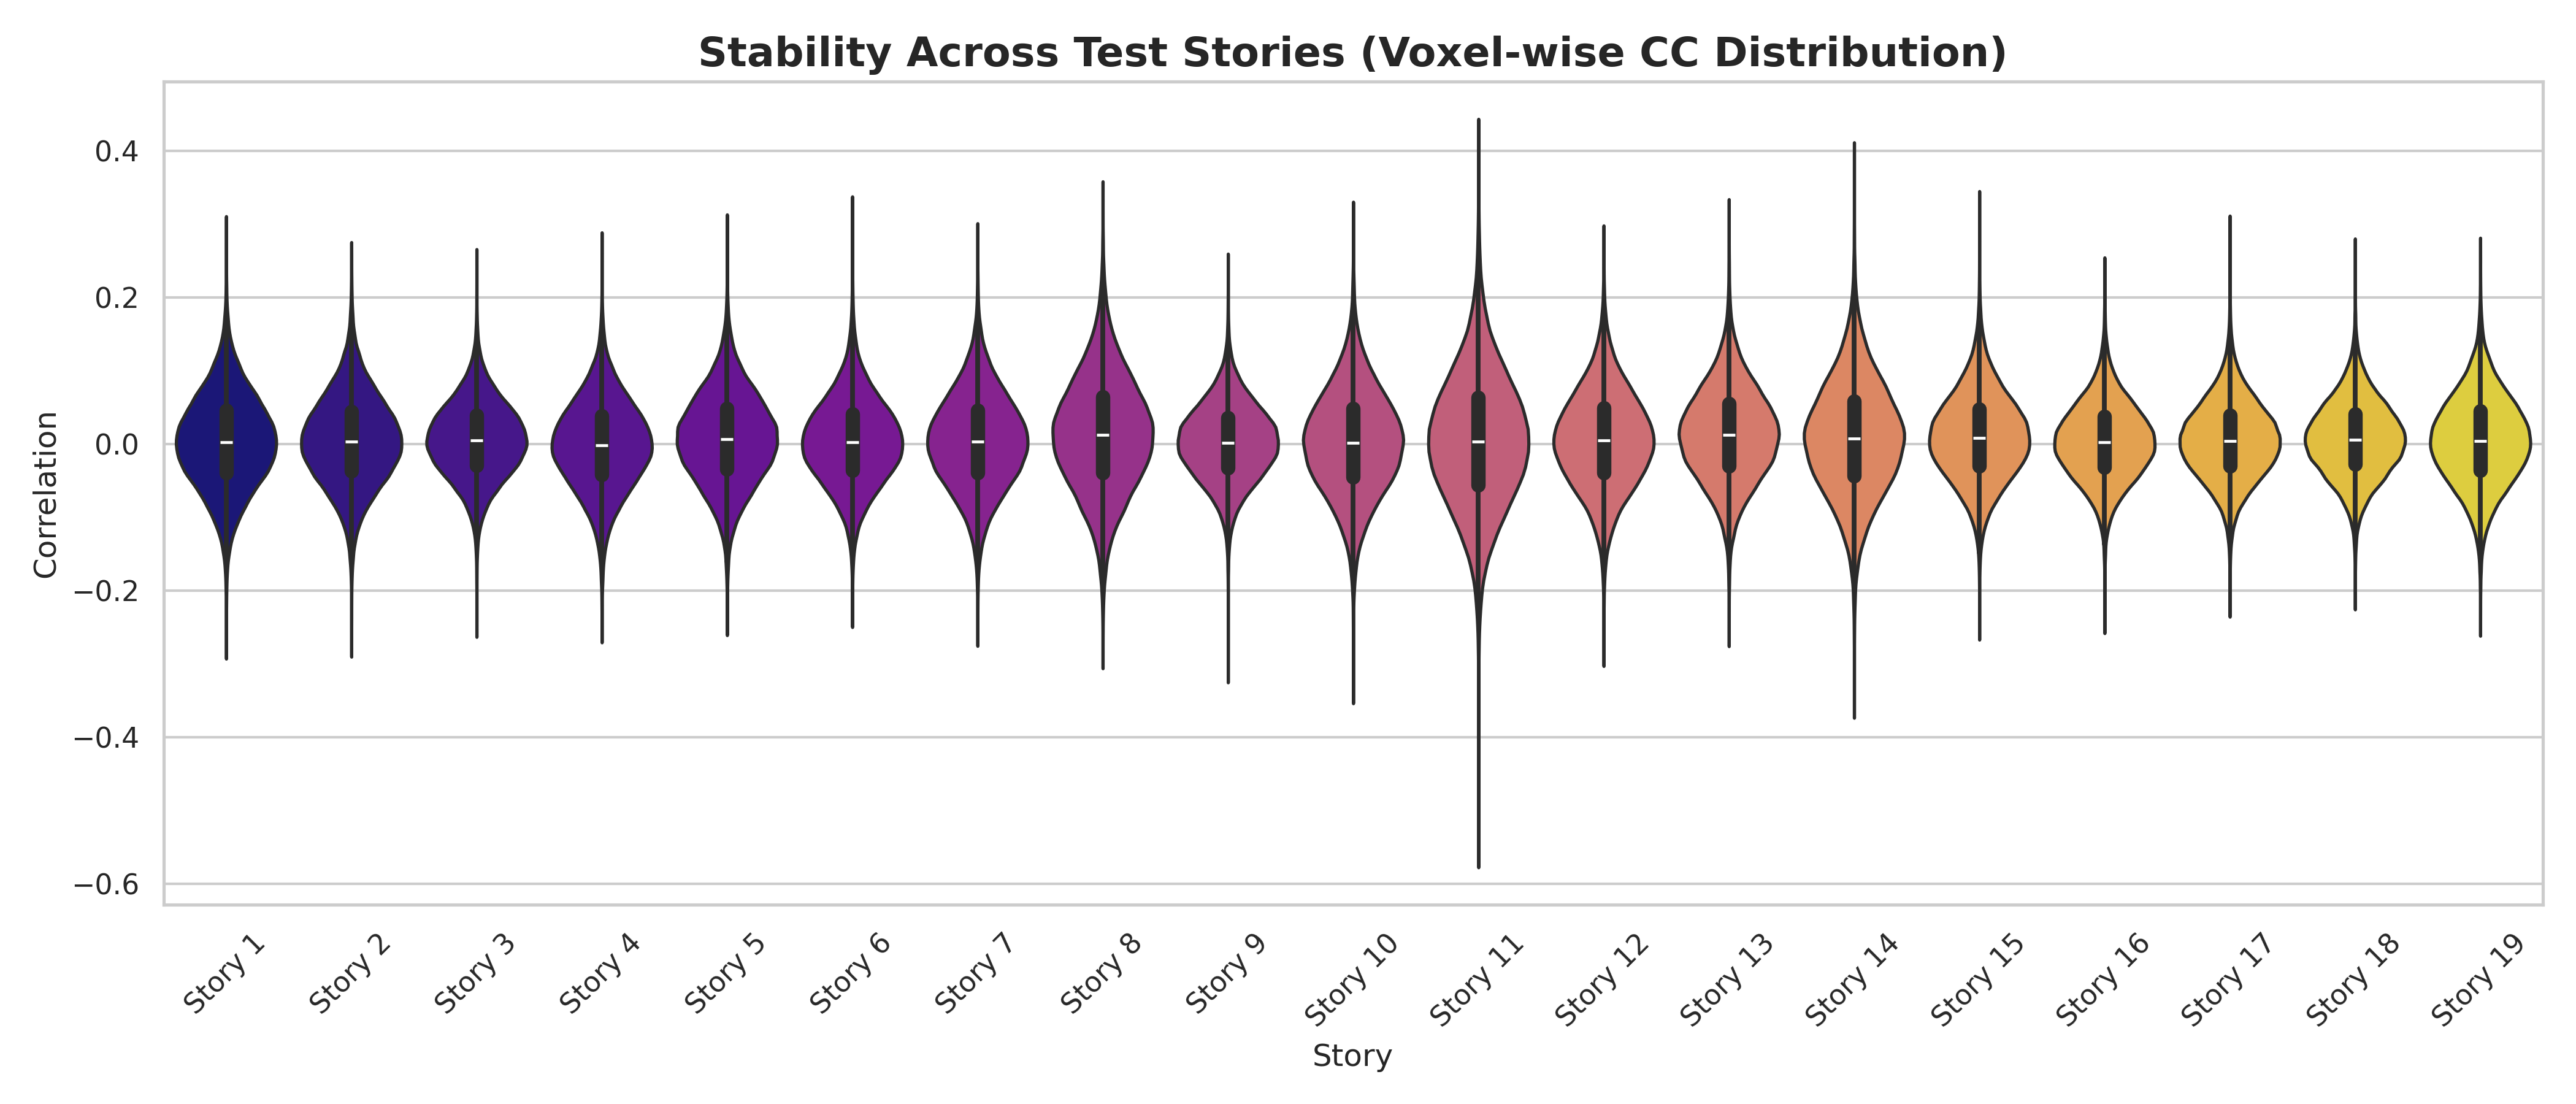
\includegraphics[width=0.9\textwidth]{figs/cc_violin_plot_stability.png}
    \caption{GloVe Correlation Coefficient Distribution}
    \label{fig:violin_glove}
\end{figure}

\newpage
\sloppy
\section{Bibliography}

[1] Jain, Shain, and Alexander G. Huth. “Incorporating Context into Language Encoding Models for fMRI.” Proceedings of the 32nd International Conference on Neural Information Processing Systems (NeurIPS), 2018, pp. 6628–6637. \url{https://proceedings.neurips.cc/paper_files/paper/2018/file/5cfb4e6e63a23722cc1a26e3027b8de2-Paper.pdf}.



\appendix

\vspace{1em} % space before
\section{Academic honesty}

\vspace{1em} % space before
\subsection{Statement}
\vspace{0.5em} % space after

We affirm our commitment to upholding the highest standards of academic integrity in all aspects of our work. We pledge to properly cite all sources, avoid plagiarism, and ensure that our contributions—whether individual or collaborative—are original and transparent. We will complete assignments independently when required and collaborate ethically, ensuring fair representation of all contributions.

We recognize that academic honesty is essential to maintaining trust and intellectual rigor within our academic community. By adhering to these principles, we strive to foster an environment of respect and integrity, understanding that any breach of these standards undermines the value of our education and the credibility of our work.


\vspace{1em} % space before
\subsection{LLM Usage}
\vspace{0.5em} % space after

\subsubsection*{Coding}
\vspace{0.5em} % space after

For the coding component of Lab 3.1 involving LLM usage, we referred to the modeling GitHub repository as a general reference. Large Language Models (LLMs) such as ChatGPT/DeepSeek were primarily utilized for debugging purposes, particularly when encountering errors or warning messages. Additionally, we consulted these models for suggestions on optimal parameters and settings to enhance the clarity and organization of our plot visualizations. However, the core coding structure and algorithmic design were primarily developed through our own discussions and understanding.

\vspace{1em} % space before
\subsubsection*{Writing}
\vspace{0.5em} % space after

For the writing component of this lab, we primarily utilized Large Language Models (LLMs) such as ChatGPT/DeepSeek to assist with grammar checking and language refinement. Despite thorough peer reviews by all four group members, it can be challenging to identify minor grammatical or stylistic errors, so LLMs served as a helpful tool for ensuring clarity and professionalism in our writing. Aside from these language enhancements, the content and conceptual understanding presented in the report were entirely based on our own knowledge, discussions, and collaborative efforts throughout the lab.

\end{document}